\documentclass[9pt]{beamer}
\usepackage{textpos}
\usepackage{gitinfo2}
\usepackage{csvsimple}
\usepackage{array,booktabs}
\usepackage{url}
\edef\masterBranch{\detokenize{master}}
\edef\gitBranch{\gitBranch}
\setbeamerfont{frametitle}{size=\large}

%fix pandoc's tightlist:https://tex.stackexchange.com/questions/257418/error-tightlist-converting-md-file-into-pdf-using-pandoc#258486
\providecommand{\tightlist}{}%
%  \setlength{\itemsep}{0pt}\setlength{\parskip}{0pt}}

% \usepackage{beamerthemesplit} // Activate for custom appearance

% \usepackage{beamerthemesplit} // Activate for custom appearance

\title{ Spacecraft Requirements, text and rationales
  \tiny{Revision: \gitDescribe, Branch: \gitBranch\\
    For access to the github repository contact edouglas@mit.edu.}}
\author{Authors}
\date{\today}

\begin{document}

%\addtobeamertemplate{frametitle}{}{
%\begin{textblock*}{200mm}(.55\textwidth,-.5cm)
%\includegraphics[height=0.6cm]{bannerlogo.png}
%\end{textblock*}}


\section{Requirement Flow}
\begin{frame}[shrink]{Requirement Flow}
\begin{figure}[htbp]
\begin{center}
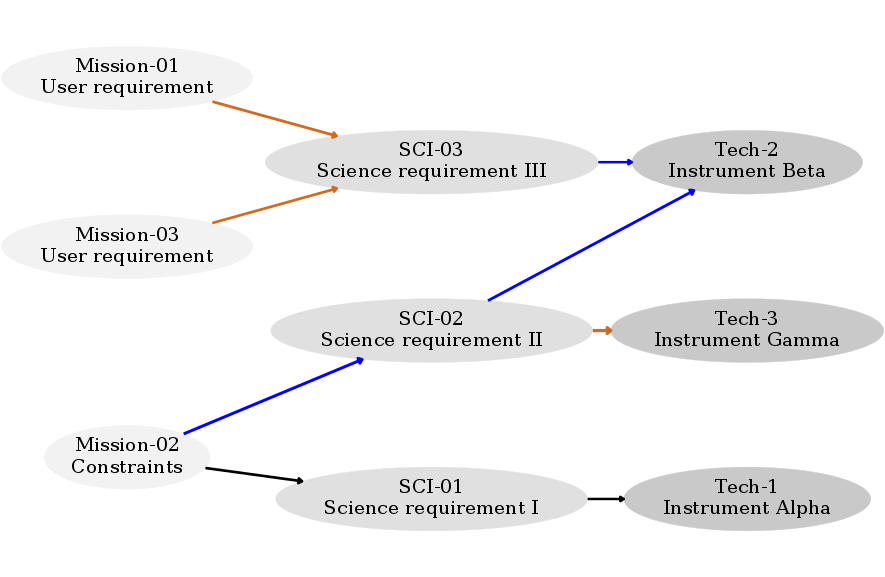
\includegraphics[width=\textwidth]{../Digraph_gv.png}
\label{default}
\end{center}
\end{figure}
\end{frame}


\frame{\titlepage}

\section[Outline]{}
\frame{Table of Contents:


\tableofcontents}
\section{Level 1}
\begin{frame}{1 Mission-01}

\emph{User requirement}

Mission level requirement A

\emph{Child links:} \href{L2.html\#SCI-03}{SCI-03}

\end{frame}

\begin{frame}{1 Mission-02}

\emph{Constraints}

Mission level requirement B

\emph{Child links:} \href{L2.html\#SCI-01}{SCI-01},
\href{L2.html\#SCI-02}{SCI-02}

\end{frame}

\begin{frame}{1 Mission-03}

\emph{User requirement}

Mission level requirement C

\emph{Child links:} \href{L2.html\#SCI-03}{SCI-03}

\end{frame}

\section{Level 2}
\begin{frame}{1 SCI-01}

\emph{Science requirement I}

Mission shall be able to perform example measurement one

\emph{Parent links:} \href{L1.html\#Mission-02}{Mission-02}

\emph{Child links:} \href{L3.html\#Tech-1}{Tech-1}

\end{frame}

\begin{frame}{1 SCI-02}

\emph{Science requirement II}

Mission shall be able to perform example measurement two

\emph{Parent links:} \href{L1.html\#Mission-02}{Mission-02}

\emph{Child links:} \href{L3.html\#Tech-2}{Tech-2},
\href{L3.html\#Tech-3}{Tech-3}

\end{frame}

\begin{frame}{1 SCI-03}

\emph{Science requirement III}

Mission shall be able to perform example measurement three

\emph{Parent links:} \href{L1.html\#Mission-01}{Mission-01},
\href{L1.html\#Mission-03}{Mission-03}

\emph{Child links:} \href{L3.html\#Tech-2}{Tech-2}

\end{frame}

\section{Level 3}
\begin{frame}{1 Tech-1}

\emph{Instrument Alpha}

Technical instrument requirement Alpha

\emph{Parent links:} \href{L2.html\#SCI-01}{SCI-01}

\end{frame}

\begin{frame}{1 Tech-2}

\emph{Instrument Beta}

Technical instrument requirement Beta

\emph{Parent links:} \href{L2.html\#SCI-02}{SCI-02},
\href{L2.html\#SCI-03}{SCI-03}

\end{frame}

\begin{frame}{1 Tech-3}

\emph{Instrument \(\Gamma\)}

Technical instrument requirement Gamma

\emph{Verification plan:}\\
test

\emph{Parent links:} \href{L2.html\#SCI-02}{SCI-02}

\end{frame}



\end{document}
